\documentclass[modern,trackchanges]{aastex631}
\bibliographystyle{aasjournal}

\usepackage[caption=false]{subfig}

\newcommand\natalienote[1]{\textbf{{\color{orange}#1}}}
\newcommand\gullynote[1]{\textbf{{\color{magenta}#1}}}
\newcommand\emilynote[1]{\textbf{{\color{cyan}#1}}}
\newcommand{\Msolar}{M$_{\odot}$}


\begin{document}
\shorttitle{Starspots on Sub-subgiant S1063}
\shortauthors{TBD}

\title{Starspots as the Cause of Underluminosity for M67 Sub-Subgiant S1063 }

\author{TBD}
\affiliation{TBD}


\begin{abstract}

We measure the starspots on a sub-subgiant.

\end{abstract}

\keywords{stars: fundamental parameters ---  stars: statistics}


\section{Introduction}\label{sec:intro}
\emilynote{This is a note from Emily.}
\natalienote{This is a note from Natalie.}
\gullynote{This is a note from Gully.}
Recent studies illuminate the important role stellar magnetic activity plays in stellar structure. This impact of stellar activity and magnetic fields is seen throughout the Hertzsprung-Russell (HR) Diagram. For example, by biasing isochronal ages of young clusters \citep{somers15}, inflating radii of active M-dwarfs \citep{2010AJ....140.1158T,2010ApJ...718..502M,2019MNRAS.483.1125J}, causing redder multiple turnoffs in stellar clusters \citep{2009MNRAS.398L..11B,2019ApJ...876..113S}, and altering the pulsation modes of red giants \citep{2020A&A...639A..63G}. As our ability to probe the detailed physics of stellar evolution continues to improve we must grapple with the complexities of stellar structure diverging from simpler theoretical expectations due to magnetic activity, which requires careful observational studies of magnetically active systems to test magnetic stellar models.

One example of the impact of magnetic activity is seen in sub-subgiant (SSG) stars, defined to be stars that lie below the subgiant branch on a cluster optical color-magnitude diagram (CMD), but are too red to be main sequence stars. These stars are commonly found in evolved open clusters and globular clusters, with 65 sub-subgiants currently identified across 17 different clusters \citep{geller17}. The majority of sub-subgiant stars are single-lined spectroscopic binaries with short orbital periods of a few days with moderate X-ray luminosities of $10^{30}$ to $10^{31}$ erg s$^{-1}$ \citep[and references therein]{geller17}.

The existence of sub-subgiants cannot be explained with typical single-star stellar evolutionary pathways. Three possible formation scenarios for sub-subgiants were put forth by \citet{geller17} and \citet{leiner17}: mass transfer in a binary system, stripping of a subgiant star envelope through a dynamical encounter, and reduced luminosity as a result of inhibited convection and large starspot covering fractions due to the presence of strong magnetic fields. \citet{leiner17} conclude that the majority of sub-subgiants are likely the result of strong magnetic fields. This interpretation is supported by the presence of H-alpha and X-ray emission and optical variability seen across the known sub-subgiant population \citep{geller17}, all observational signatures of magnetic activity and the presence of starspots. 

Ideally we would directly measure the radius and internal magnetic field to calibrate how the star inflates as a function of convective efficiency, and the positions of SSGs could be explained.  In practice these quantities are difficult to measure at the precision required to demonstration inflation on single magnetically active systems, though aggregate populations have shown evidence for magnetic inflation \citep{2018AJ....155..225K,2018MNRAS.476.3245J}. Starspots have become a rich observational proxy for gauging the evolutionary state of stars that may be magnetically inflated, without needing to estimate magnetic field strengths.

The portion of the stellar surface covered with starspots is related to the amount of magnetic activity. The mere existence of starspot modulation betrays magnetic activity in stars.  Starspots rupture the otherwise-pristine photospheric boundary conditions that regulate energy loss from stars.  Starspots emit light of their own that can be captured and analyzed to quantify the impact of such boundary condition changes.  

A full accounting of starspots requires careful consideration of geometrical degeneracies.  Monochromatic light curves can indicate spotted stars \citep{2014ApJS..211...24M} but can only provide a lower limit on the differential spot coverage between the most and least spotted hemispheres. Longitudinally symmetric starspot geometries evade detection in monochromatic lightcurves alone \citep{2019AJ....157...64L}. Measuring the spot configuration typically requires Doppler imaging or interferometry studies restricted to only the brightest and most nearby sources \citep{roettenbacher16}.  Disk-integrated covering fractions can be obtained from TiO band observations \citep{oneal96,fang2016,2019AJ....158..101M}. Testing the next era of stellar activity models requires precision methodologies to measure spot-covering fractions of a larger number of targets, including sub-subgiants. 

Starspots emit a spectrum of their own at a lower temperature and with distinct absorption features compared to the ambient photosphere. The observed spectrum is a composite of the spot and photosphere spectra and can therefore be deconvolved. This deconvolution constrains the spot-covering fraction as well as the spot and photosphere temperatures. This is possible by performing a two-temperature probabilistic spectral decomposition using the spectral inference framework \texttt{Starfish} \citep{czekala15}, recently extended to support composite spectra \citep{gullysantiago17}. The resulting spot characterization can be used to anchor light curve information, providing insight into the overall stellar activity level and constraining the long-term spot coverage \citep{neff95}. This strategy only requires high-resolution echelle spectroscopy and photometric monitoring, dramatically increasing the number of sources for which we can observationally constrain spot-covering fractions.

In this paper we demonstrate the power of this methodology by focusing on a single sub-subgiant system, S1063 in the open cluster M67. This system is a prototypical sub-subgiant star, with an single-lined spectroscopic orbital period of 18.4 days \citep{geller17}, an X-ray luminosity of $1.3\times10^{31}$ erg s$^{-1}$ \citep{vandenberg99}, and a variable light curve in \textit{K2} and ASAS-SN (Section~\ref{sec:K2lightcurve}). \emph{Gaia} DR2 astrometry \citep{2016A&A...595A...1G, 2018A&A...616A...1G} indicates a parallax ($1.17\pm0.025 \;$mas) and proper motion for S1063 (\emph{Gaia} DR2 604921030968952832) consistent with other M67 members, and approaching 100\% membership probability \citep{2018ApJ...869....9G}. We present our observational data products in Section~\ref{sec:observations} and subsequent analysis in Section~\ref{sec:analysis}. Our results are given in Section~\ref{sec:results} with Discussion in Section~\ref{sec:discussion}. Finally, our conclusions are outlined in Section~\ref{sec:conclusions}.


\section{Observation and data reduction}
\label{sec:observations}


\subsection{IGRINS observations}
A high resolution spectrum of S1063 was acquired with the $R=45,000$ Immersion Grating Infrared Spectrograph \citep[IGRINS;][]{park14} at UT 2015-04-26 $03^h29^m$ at the $2.7\;$m Harlan J. Smith Telescope at McDonald Observatory.  Eight 600-second individual exposures were acquired in an ABBA nod pattern at an airmass of 1.2.  The sky emission lines and telluric lines were removed with the IGRINS Pipeline Package  \citep[PLP;][]{jaejoonlee16} and a reference A0V star acquired nearby in time and airmass.
The $H-$band spectra exhibited a signal-to-noise ratio of approximately $50$ per pixel.
The $K-$band spectra possessed low $S/N$ and were excluded from further analysis.

\begin{figure*}[ht]
  \centering
  \begin{tabular}{ccccc}
    \subfloat{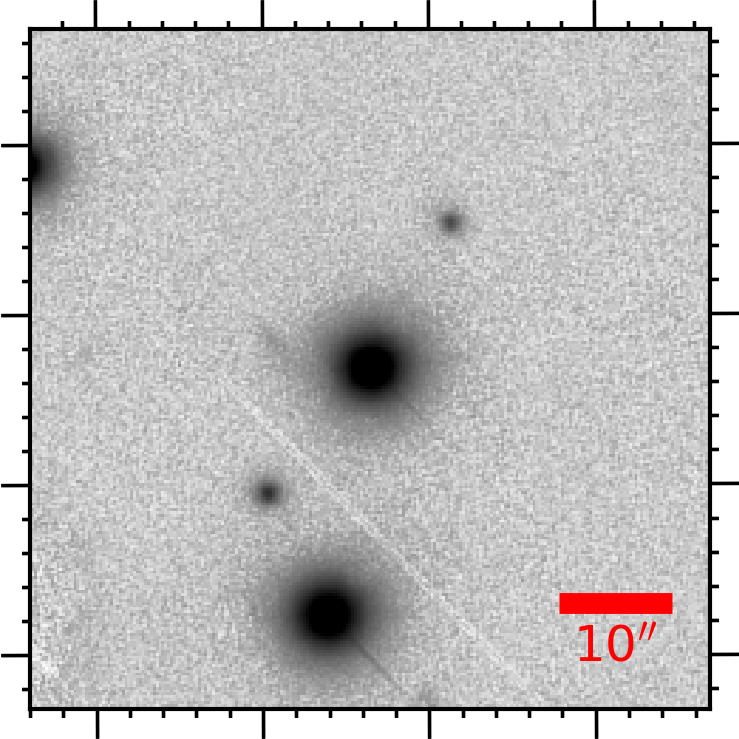
\includegraphics[width=1in]{figures/S1063_60x60arcsec_PS1_g.png}} &
    \subfloat{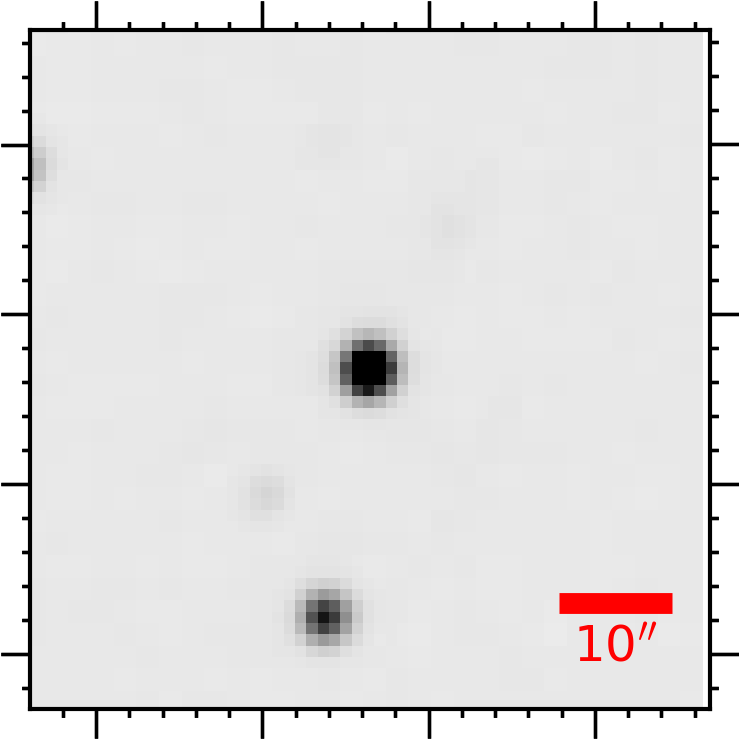
\includegraphics[width=1in]{figures/S1063_60x60arcsec_2M_J.png}} &
    \subfloat{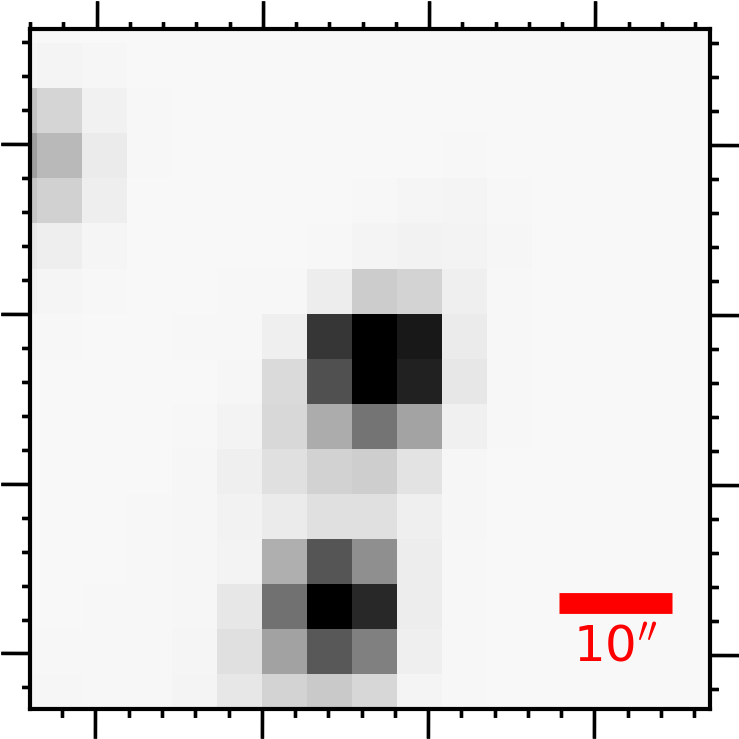
\includegraphics[width=1in]{figures/S1063_60x60arcsec_K2_C5.png}} &
    \subfloat{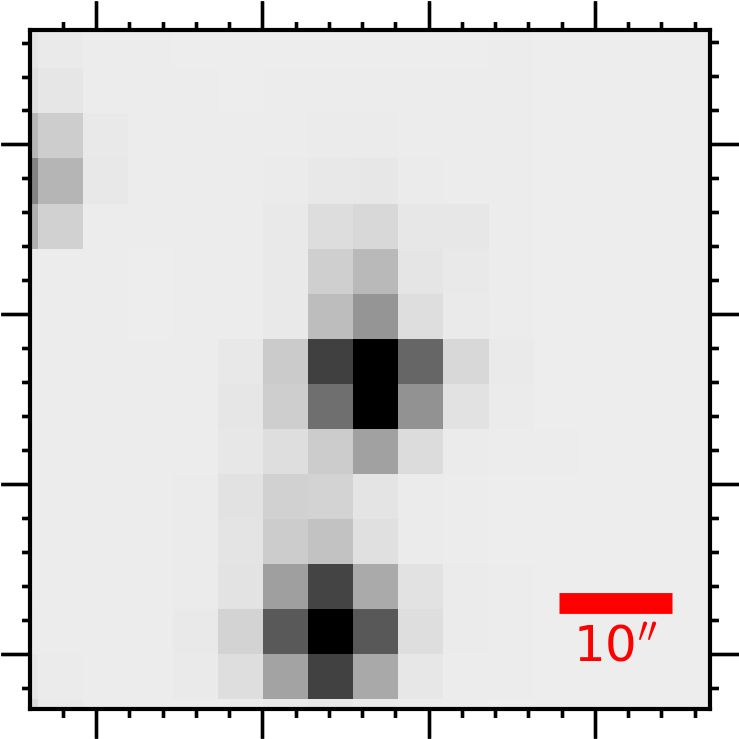
\includegraphics[width=1in]{figures/S1063_60x60arcsec_K2_C16.png}} &
    \subfloat{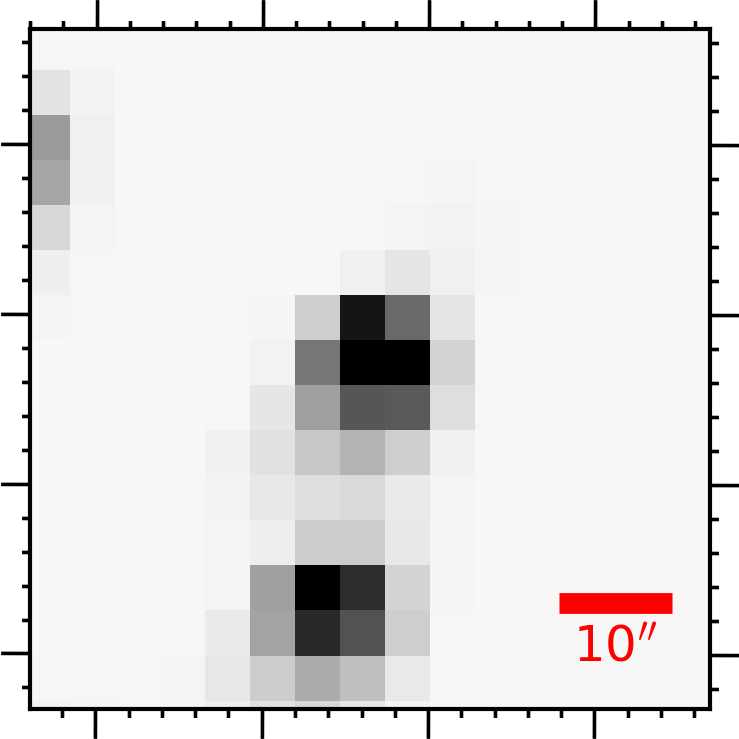
\includegraphics[width=1in]{figures/S1063_60x60arcsec_K2_C18.png}} \\
  \end{tabular}
\caption{Imaging of S1063 in $60'' \times 60''$ postage stamps. \emph{left-to-right:} Pan-STARRS $g$-band co-added image contemporaneous with C16; 2MASS $J-$band; K2 Campaigns 5, 16, 18 from Full Frame Images.  S1063 is sufficiently separated from nearby sources in the coarse \emph{Kepler} imaging.}
\label{fig:imaging}
\end{figure*}

\subsection{K2 superstamp lightcurves}
The \emph{Kepler} spacecraft targeted S1063 (EPIC 211414597) during the \emph{K2} mission \citep{howell14} in Campaigns 5, 16, 18 as part of the M67 superstamps.  The instrumental point spread function (PSF) of S1063 fell entirely within the oversized K2 target pixel files in Campaign 5 (K2 Custom Aperture ID 200008674, channel 13) and Campaign 18 (K2 Custom Aperture ID 200233338).  Aperture photometry was conducted with interactively-assigned custom apertures using the \texttt{lightkurve.interact()} feature \citep{geert_barentsen_2019_2565212}. The apertures were chosen to minimize flux-loss out of the aperture due to spacecraft-induced image motion, while avoiding low-$S/N$ pixels and the wings of adjacent PSFs.  The Campaign 16 source PSF overlapped the edge of Custom Aperture ID 200200534, therefore a mosaic of adjacent superstamps was assembled before conducting aperture photometry.
We detrended motion-induced image artifacts with the Self Flat Field algorithm \citep{vanderburg14} implemented in \texttt{lightkurve}.  Postage stamp images are shown in Figure \ref{fig:imaging}.


\subsection{Ground-based photometric monitoring}
We retrieved All-Sky Automated Survey for Supernovae \citep[ASAS-SN;][]{shappee14} lightcurves from the Sky Portal \citep{2017PASP..129j4502K}.  The lightcurves contained 758 epochs of $V-$ band photometry spanning 2013-2018 (source ASASSN-V J085113.44+115139.7) and 823 epochs of $g-$band photometry spanning mid-2017--2018.  The $\sim8''$ ASAS-SN pixels may cause some PSF blending of the nearby-albeit-fainter source seen at the bottom of Figure \ref{fig:imaging}.  The pixel images were not available to evaluate the extent of blending.

\subsection{Inter-campaign relative photometry with K2 Full Frame Images}\label{sec:K2lightcurve}

Stellar activity cycles on S1063 can secularly change the stellar brightness on timescales comparable to the separation of the three campaigns of \emph{K2} observations.  The comparison of flux levels among repeated \emph{K2} campaigns requires accounting for detector responsivity degradation on these same timescales.  The absolute sensitivity of the \emph{Kepler} detector pixels decay at $\sim1 \%\;\textrm{yr}^{-1}$ due to sudden pixel sensitivity dropouts and other environmental lifetime factors \citep{montet17}. 

To account for sensitivity changes, we calibrate the system-integrated throughput for \emph{Kepler} detector channels including the M67 field for Campaigns 5, 16, and 18. We measure aperture photometry for approximately 2000 isolated reference stars from the Full Frame Images, keeping only those stars that were observed in all three campaigns. Compared to Campaign 5, the reference stars have a median flux of $93.9\pm4.2\%$ in Campaign 16 and a median flux of $98.2\pm2.8\%$ in Campaign 18. Campaigns 5 and 18 were observed on the same detector channel while a different detector channel was used for Campaign 16, therefore these offsets are not a significant measure of detector degradation across campaigns. 

 

\begin{figure*}[ht]
    \centering
    \begin{tabular}{cc}
      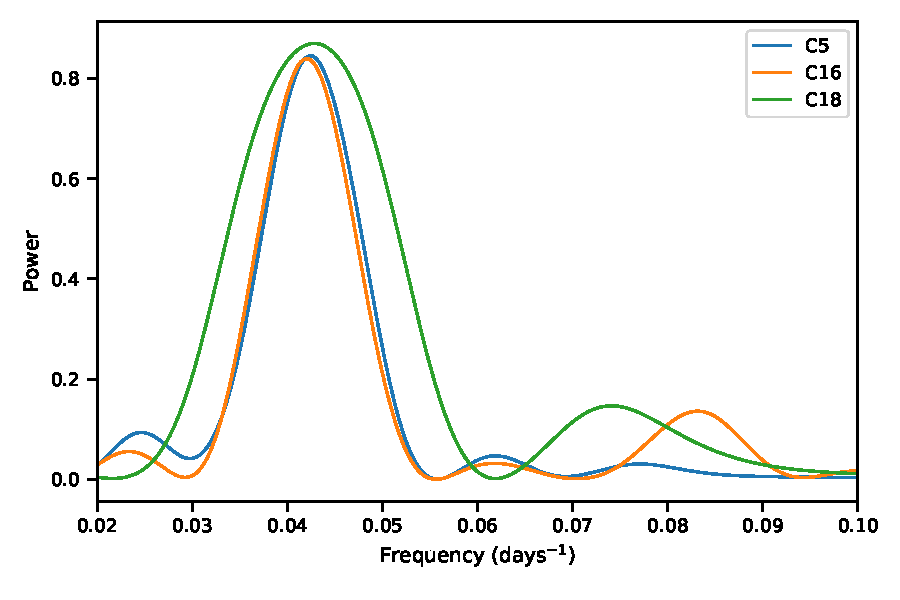
\includegraphics[width=3in]{figures/AllCampaigns_Periodogram.pdf}   & 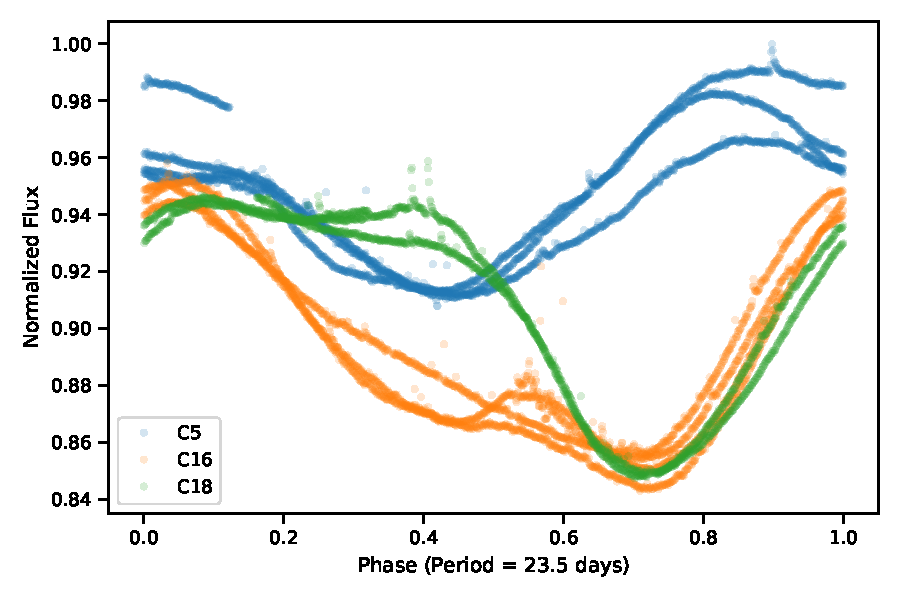
\includegraphics[width=3in]{figures/AllCampaigns_Phased_Lightcurve.pdf}  \\
    \end{tabular}
    \caption{On the right, a Lomb-Scargle Periodogram of the light curve for each \emph{K2} campaign and on the left, the corresponding phased \emph{K2} light curves. The average period associated with maximum power across all three campaigns is P = 23.5 days. \deleted{The phased light curves indicate the most spotted hemisphere occurred around a rotation phase of 0.4 during C5 (shown in blue) but shifted to a rotation phase of approximately 0.7 in C16 and C18 (shown in purple and green, respectively). This is suggestive of the spot morphology of S1063 shifting over this 2.5-year period.} \explain{How precisely do we have to know the period to confidently detect a phase change?} }
    \label{fig:periodogram}
\end{figure*}


\begin{figure*}[ht]
  \centering
  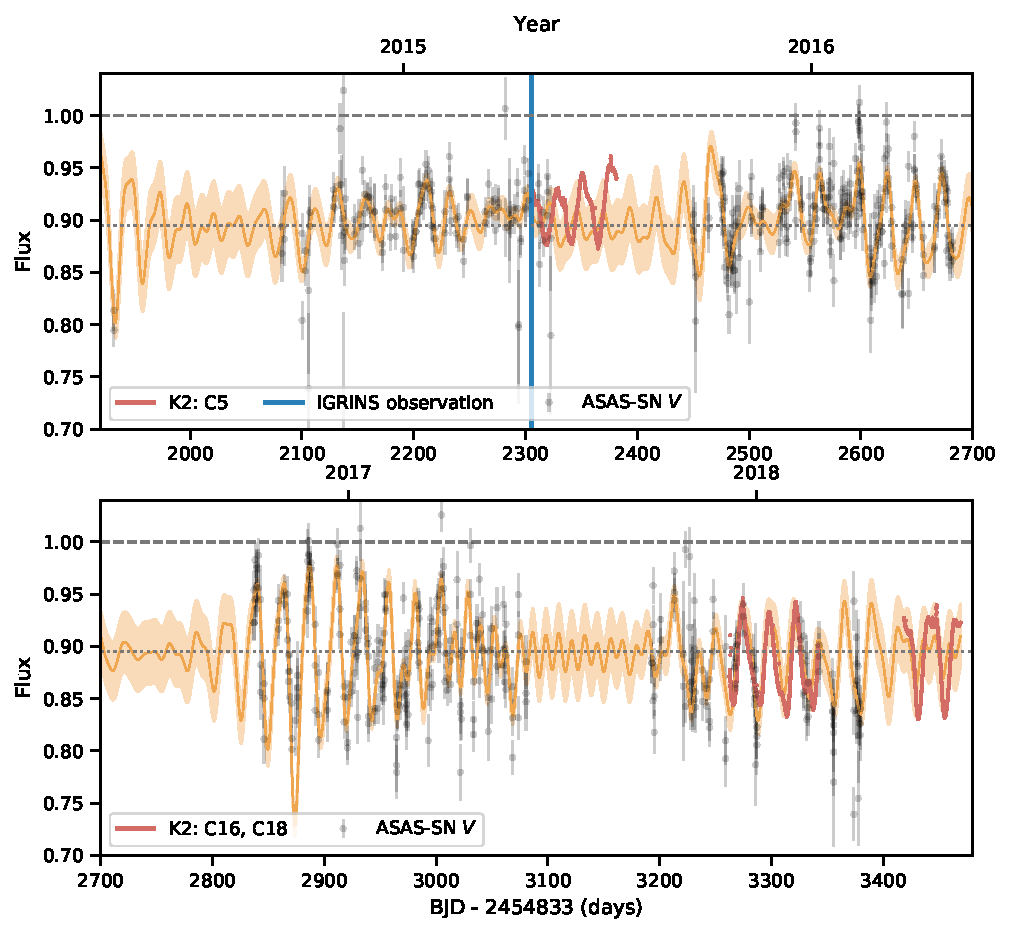
\includegraphics[width=0.95\textwidth]{figures/2020_K2_ASASSN_lcurve_2panel.pdf}
\caption{Four year lightcurve for S1063, normalized to a maximum flux of 1.00 as denoted by the gray dashed line. The mean flux of 0.895 is shown with the gray dotted line.  \emph{K2} Campaigns 5, 16, and 18 (densely-sampled red points) and ASAS-SN $V-$band (coarsely-sampled gray points) show approximately $5-17\%$ peak-to-valley photometric variations indicative of secularly evolving surface coverage of starspots.  The orange line shows a damped, driven harmonic oscillator \emph{celerit\`e} model \citep{2017AJ....154..220F} trained on the K2 and ASAS-SN data, and then applied to the noisy ASAS-SN points, with a standard-error uncertainty band in shaded orange. The vertical blue bar in mid-2015 indicates the epoch of IGRINS data acquisition, which shows an approximate $8\%$ flux deficit compared to global maximum flux in early 2017.}
\label{fig:lightcurve}
\end{figure*}


\section{Analysis}
\label{sec:analysis}

%INTRO TEXT:
%Starspots emit a spectrum of their own at a lower temperature and with distinct absorption features compared to the ambient photosphere. The observed spectrum is a composite of the spot and photosphere spectra and can therefore be deconvolved. This deconvolution constrains the spot-covering fraction as well as the spot and photosphere temperatures. This is possible by performing a two-temperature probabilistic spectral decomposition using the spectral inference framework \texttt{Starfish} \citep{czekala15}, recently extended to support composite spectra \citep{gullysantiago17}. The resulting spot characterization can be used to anchor light curve information, providing insight into the overall stellar activity level and constraining the long-term spot coverage \citep{neff95}. This strategy only requires high-resolution echelle spectroscopy and photometric monitoring, dramatically increasing the number of sources for which we can observationally constrain spot-covering fractions. 

Constraining starspot covering fraction for stars such as S1063 requires a careful combination of light curve interpretation and spectral analysis, using spectral decomposition tools such as \texttt{Starfish} \citep{czekala15} to benchmark epochs of starspot coverage in long-term photometric monitoring. 

\subsection{Joint modeling of ASAS-SN and \emph{K2} Lightcurves}
In order to characterize the long-term behavior of S1063 we jointly modeled the ASAS-SN and K2 lightcurves as a damped, driven Simple Harmonic Oscillator (SHO) Gaussian Process (GP) with \texttt{celerit\`e} \citep{2017AJ....154..220F}, revealing periodicity and secular changes in flux levels over a multi-year timeframe.  This strategy offers flexibility to cope with windowing effects and the high dynamic range in data sampling and quality available across ASAS-SN and \emph{K2}.  The ASAS-SN $V$-band and \emph{K2} photometric band share significant overlap and are treated as the same for this analysis. 

 We tuned a two-period GP model, with the harmonic component possessing roughly half the period $P_H\sim12.5\;\mathrm{d}$ of the fundamental period $P_0=23.5\;\mathrm{d}$.  The harmonic overtone frequency can be seen by eye in Figure \ref{fig:lightcurve}, as the \emph{K2} lightcurves appear more complex than a pure sine wave.  Each periodic GP term also possessed correlation amplitude and SHO quality factor which we consider nuisance parameters for the purpose of this fitting.  We found broadly consistent values when \emph{K2} lightcurves were fitted on a per-campaign basis.  We then fit the three campaigns \emph{simultaneously} in the following way.  We set the overall vertical registration of the \emph{K2} lightcurves such that the ASAS-SN and Campaign 16 trends match, since M67 was contemporaneously observable from the ground for the entire duration of K2 Campaign 16. The uncertainty in the inter-campaign offsets calculated in Section~\ref{sec:K2lightcurve} is larger than the internal precision of the \emph{K2} photometry, so we adjust the Campaign 5 data within the offset uncertainty to match the approximately one week of temporal overlap with ASAS-SN.  We added an additional non-periodic secular trend GP component to capture the campaign-to-campaign mean-level variation, also considered a nuisance parameter.

Finally, we evaluated the trained GP model at the location of the ASAS-SN photometry, and at windows lacking data altogether.  This trend appears in Figure \ref{fig:lightcurve} as the dark orange line with an orange standard confidence region.  This trendline guides the eye to see broad secular changes to the amplitude encoded in the noisy ASAS-SN data, with a global maximum peak-to-valley amplitude of 17\% occurring near 2017 January, and global minimum peak-to-valley of 3\% occurring near to the time of the IGRINS measurement. 


\subsection{IGRINS two-temperature spectral decomposition}

Even a single epoch of IGRINS observations provides an opportunity to constrain the spot covering fraction of S1063 that can be used as a benchmark for interpreting the long-term flux variation apparent in Figure~\ref{fig:lightcurve}. We performed a two-temperature probabilistic spectral decomposition on the IGRINS $H-$band spectrum.  We applied the spectral inference framework \texttt{Starfish} \citep{czekala15}, recently extended to support composite spectra comprised of mixtures of two distinct photospheric components \citep{gullysantiago17}.  Here, the two temperature components are labeled as $T_{\mathrm{spot}}$ and $T_{\mathrm{amb}}$ for the starspot and ambient photospheric emission, respectively, with a filling factor $f$ defined as the ratio of disk-integrated projected surface area of the spot groups to the projected area of the star.

We employed the \texttt{PHOENIX} precomputed synthetic model grid \citep{husser13} with grid ranges of $3000 < T_{\mathrm{eff}} \; (\textrm{K}) < 5300 $, $3 < \log{g \;(\textrm{cm/s})}  < 4 $, and $ -0.5 <  [\mathrm{Fe}/\mathrm{H}] <0.5$.  We trained the spectral emulator \citep{czekala15} on this grid range, while preserving the absolute model mean fluxes to enable accurate flux comparison between two spectra of disparate characteristic temperatures.  This new approach offers improved accuracy over the scalar flux interpolated approach introduced in Appendix A of \citet{gullysantiago17}, especially for such a large dynamic range in effective temperature.  The spectral emulator approach also propagates the uncertainty attributable to the coarsely sampled \texttt{PHOENIX} models.

The pre-defined grid ranges place uniform priors over their domain.  Additionally, a threshold of 4500 K separated the allowed domains for the spot and ambient temperatures, yielding uniform priors $3000 < T_{\mathrm{spot}} \; (K) < 4500 $ and $4500 < T_{\mathrm{amb}} \; (K) < 5300$.

\subsubsection{MCMC convergence and posterior predictive checks}

Each IGRINS $H$-band spectral order was fit independently, yielding over 20 individual sets of MCMC posteriors.  We employed \texttt{emcee} \citep{foreman13} with 5000 samples and 40 walkers, spot-checking the MCMC chains for signatures of steady-state posterior probability distributions suggestive of convergence.  Some orders did not pass our convergence criteria, usually due to poor initialization of nuisance parameters or overfitting.  Furthermore, the radial velocity $v_z$ and projected rotational broadening $v\sin{i}$ were spot-checked to verify both consistent values among spectral orders as well as posterior distributions indicative of information-rich spectral orders.  Some relatively feature-free spectral orders such as $m=103$ did not offer enough constraining power to derive meaningful results in the face of multiple sources of degeneracy.  Collectively, these discrepant or uninformative spectral orders were removed from future analysis, yielding a total of nine preserved spectral orders, shown in Figure \ref{fig:IGRINS_spectra3x3}. All spectral orders were consistent with a $v\sin{i}=10 \;\mathrm{km/s}$, with typical per-order $1-\sigma$ uncertainties of $0.2-1.0 \;\mathrm{km/s}$.  The per-order estimates for radial velocity were all consistent with $v_z=44\;\mathrm{km/s}$ at the measurement epoch, uncorrected for barycentric motion.

\begin{figure*}[ht]
 \centering
 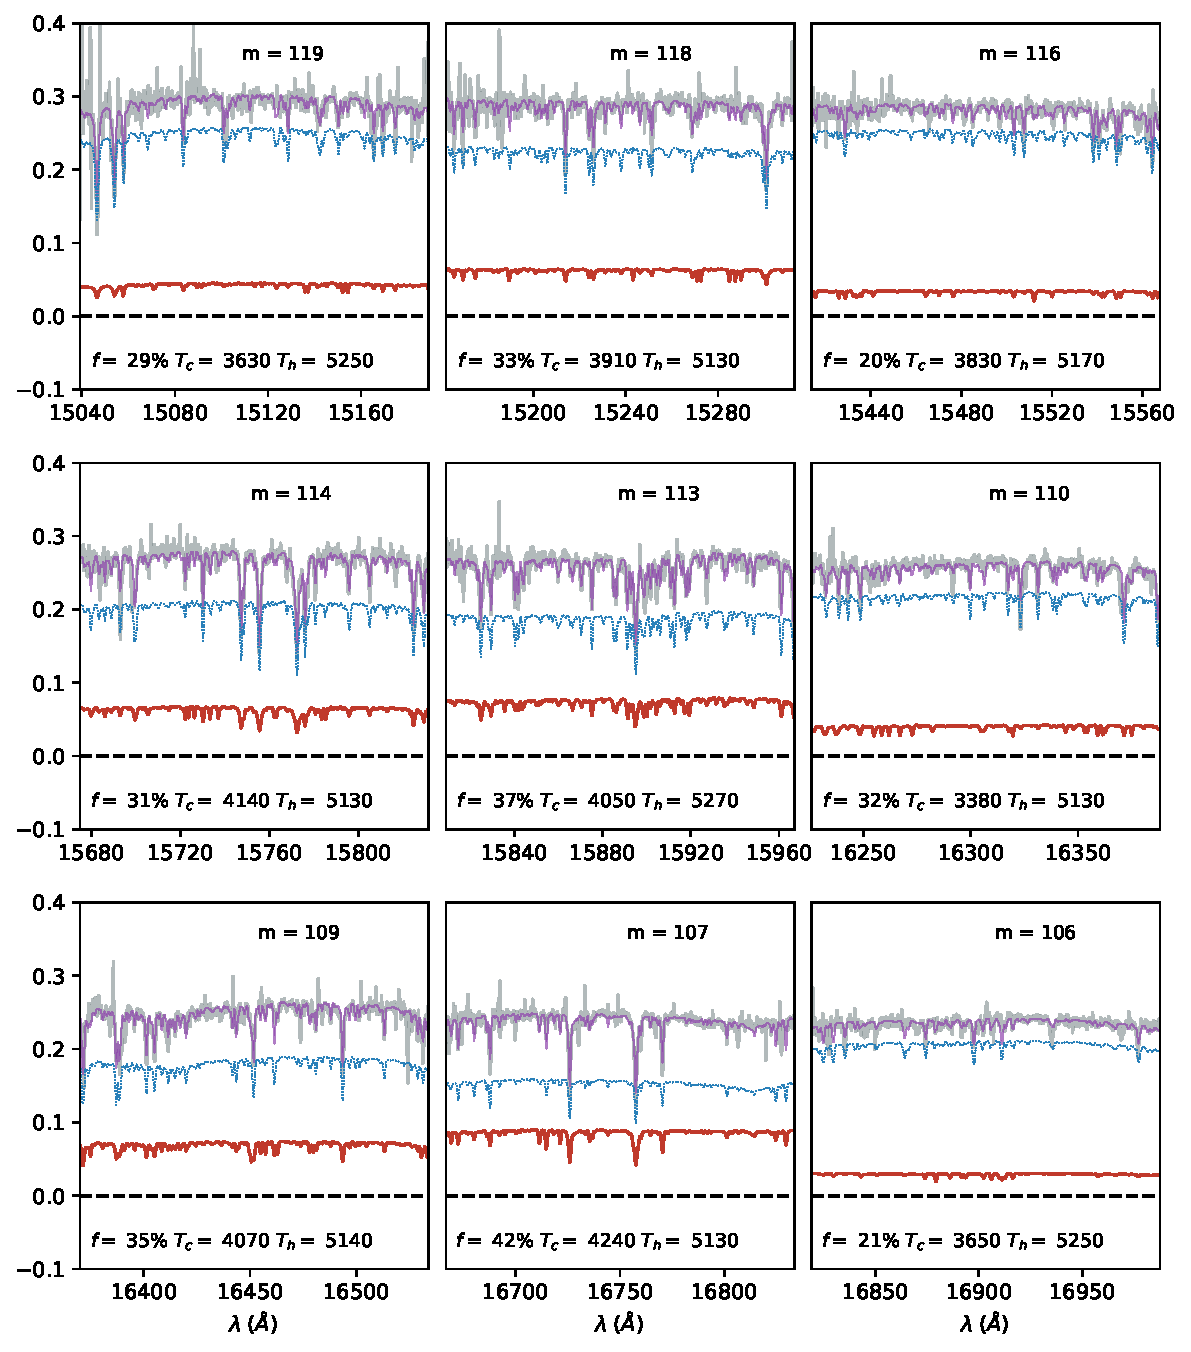
\includegraphics[width=0.90\textwidth]{figures/H_band_spectra_3x3.pdf}
 \caption{Nine $H-$band IGRINS echelle orders showing two-component spectral decomposition of collective starspot photospheric emission, labeled with the corresponding order number $m$.  The starspot spectrum (thick red line) and ambient photosphere spectrum (dotted blue line) combine to form the composite spectrum (solid purple line) that resembles the observed spectrum (thick gray line).  The starspot and ambient components can share similar spectral structure, leading to a range of filling factors and temperatures ranges with nearly equivalent composite spectra; here we present a single random draw from the MCMC posterior, not a ``best fit''.  The cool and hot temperatures $T_{\textrm{s}}$ and $T_{\textrm{amb}}$ for each draw show variety consistent with the fitting uncertainty. The corresponding spot filling factor, $f_{\textrm{s}}$, is also shown for each specific random draw. Unexplained spectral structure and over- and under- fitting of spectral lines arises from a combination of PHOENIX model imperfections, possible magnetic Zeeman broadening, and other model mis-specifications.}
 \label{fig:IGRINS_spectra3x3}
\end{figure*}

%\subsubsection{Consistency of stellar characterization}
%Vsini is similar to before and radial velocity is what we expect given orbital phasing (NEED TO DO THE PHASING).


%TODO: Analysis of near-IR flux contribution from binary companion
%TODO: Limits on companion types


\section{Results}
\label{sec:results}

\subsection{Spot temperature and filling factor}
\label{sec:starfishresults}
Using the \texttt{Starfish} spectral inference results we investigate the joint constraints on spot temperature and filling factor, marginalized over all other uncertainties in stellar properties and fitting hyper-parameters (such as Starfish-derived Gaussian Process correlation length and amplitude and continuum fitting polynomials). In Figure~\ref{fig:tspot_fillingfactor3x3} we show 2-dimensional posterior distributions of filling factor and spot temperature of the last 1000 samples thinned by a factor of 10 from all 40 \texttt{emcee} walkers for the nine orders with accepted fits. The orders show broad agreement between spot temperature and filling factor. Across all nine orders, the median filling factor value is 32\% with a standard deviation of 7\%, with a corresponding spot temperature of $4000 \pm 200$ K. The ambient photosphere temperature associated with this spot signature varies from order-to-order and is broadly consistent with a range of temperatures between 5000 K and 5300 K, with a best guess value of $5200$ K.  These values are broadly consistent with a spectroscopic temperature of 5000 K determined by \citet{mathieu03} determined from visible-wavelength spectra.  Visible wavelength spectra principally perceive the ambient photosphere, due to the near-zero starspot contrast at those wavelengths.  Therefore the most reliable ambient photosphere estimate likely stems from the visible-based measurement, and not our near-IR-based estimate.

\subsubsection{Light curve interpretation}
The ASAS-SN and \textit{K2} C5 data of S1063 (Figure~\ref{fig:lightcurve}) indicate that the IGRINS observation was coincidentally acquired near its modest local maximum at an overall flux level of 91.2\%. This is close to the overall 89.5\% mean flux level, where the 100\% flux level is equal to the global maximum over the four-year period covered by ASAS-SN and \textit{K2}. The lightcurve exhibits relatively modest variability at the time of the IGRINS observations with merely 3\% peak-to-valley variation compared to its global largest variation of almost 17\% as observed around 2017 January.  

For a first-order interpretation of light curve amplitudes, we posit that the lightcurve is starspot-dominated as opposed to facula-dominated.  Under this assumption, minimum light corresponds to the largest blockage of ambient flux and therefore the largest starspot coverage on the instantaneous hemisphere projected towards the observer \cite{basri18}.  Maximum light corresponds to the moments with the least---\emph{but not necessarily zero}---starspot coverage.  

If S1063 was spot-free at the time of the global lightcurve maximum the epoch of IGRINS observation would correspond to starspots blocking 8.8\% of the total instantaneous stellar flux (100\% $-$ 91.2\% $=$ 8.8\% blocked flux at the time of observation), assuming non-emitting starspots. However, starspots are emitting and effectively filling in some of the light that is ``blocked''.  This non-zero starspot emission demands that the spot covering fraction must be greater than 8.8\% at the time of the IGRINS observation. Adopting an ambient photosphere temperature of 5200 K and a spot temperature of 4000 K, the projected spot coverage of S1063 must be at least 13\% to account for the 8.8\% flux loss in the $V$-band. 

This 13\% spot coverage is a minimum value based on an assumption that the maximum lightcurve flux results from an un-spotted star. Our spectral inference results indicate the spot coverage at the time of the IGRINS observation was, in fact, 32\%. This suggests that at maximum light over this 4-year period the spot coverage of S1063 was approximately 20\%, and not zero as a first-order interpretation of the light curve would imply. 

The presence of starspots at the light curve maximum acts as a starspot baseline for interpreting the lightcurve. Over the 4-years shown in Figure~\ref{fig:lightcurve}, the average flux variation is approximately 5\%, corresponding to an average spot covering fraction variation from each observed hemisphere of $\pm$8\%. The lightcurve exhibits a global flux minimum 10\% lower than the flux at the time of the IGRINS observation, requiring a spot filling factor close to 45\% on the projected hemisphere at that time.  

We therefore determine that over the time period from 2014--2018 S1063 has possessed a range of 20--45\% coverage fraction of spots, with an average close to 30\%. The IGRINS observation occurring near the mean global flux level fortuitously allows a robust characterization of the average state of S1063. These numbers possess formal uncertainties in the few percent range, and additional uncertainties from our reliance on spectral models.  But broadly speaking, our result is firm under our assumptions--- S1063 has a large persistent starspot population that ebbs and flows in its longitudinal symmetry, resulting in variation in the peak-to-valley modulation, but always possesses an approximately 30\% spot covering fraction.

\begin{table}[]
\label{tab:s1063parameters}
\caption{S1063 Surface and Stellar Parameters}
\begin{tabular}{llcccc}

  &         & Spot temp  & Filling factor & Ambient temp & Radius  \\
   &        &  (K) & (\%) &  (K) & ($R_{\odot}$) \\ \hline
\multicolumn{3}{l}{\textit{Spectroscopic Constraints:}}  \\
\phantom{EEE} & This work     & $4000\pm200$  & $32\pm7$    & 5200 &   3.7--4.6     \\
& \citet{mathieu03} &  ...    &  ...    &     5000    &  2.4  \\
\multicolumn{3}{l}{\textit{Photometric Constraints:}} \\
& SPOTS models$^{a}$  &      &  50--80    &         &        \\
& \citet{leiner17} & ... & ... & 4500$^\textrm{b}$ & 2.8--3.1 \\
& & 3500$^\textrm{c}$ & 40 & 4750 & 3.4 \\
\hline
\multicolumn{6}{l}{$^{a}$Section~\ref{sec:model_comparison}, from \citet{somers20}.} \\
\multicolumn{6}{l}{$^{b}$Unspotted model.} \\
\multicolumn{6}{l}{$^{c}$Model assuming 40\% spot coverage with a spot temperature contrast of $\sim$1000 K.}
\end{tabular}
\end{table}

%text from Leiner et al. 2017: Similarly, adding a spot to 13008 changes the best-fit parameters to 4750 K and 3.4 RSun, closer to the 5000 K spectroscopic temperature (Mathieu et al. 2003). --is this also at 40% spot covering fraction like 15028 in the previous paragraph?

 \begin{figure*}[ht]
   \centering
   \begin{tabular}{ccc}
     \subfloat{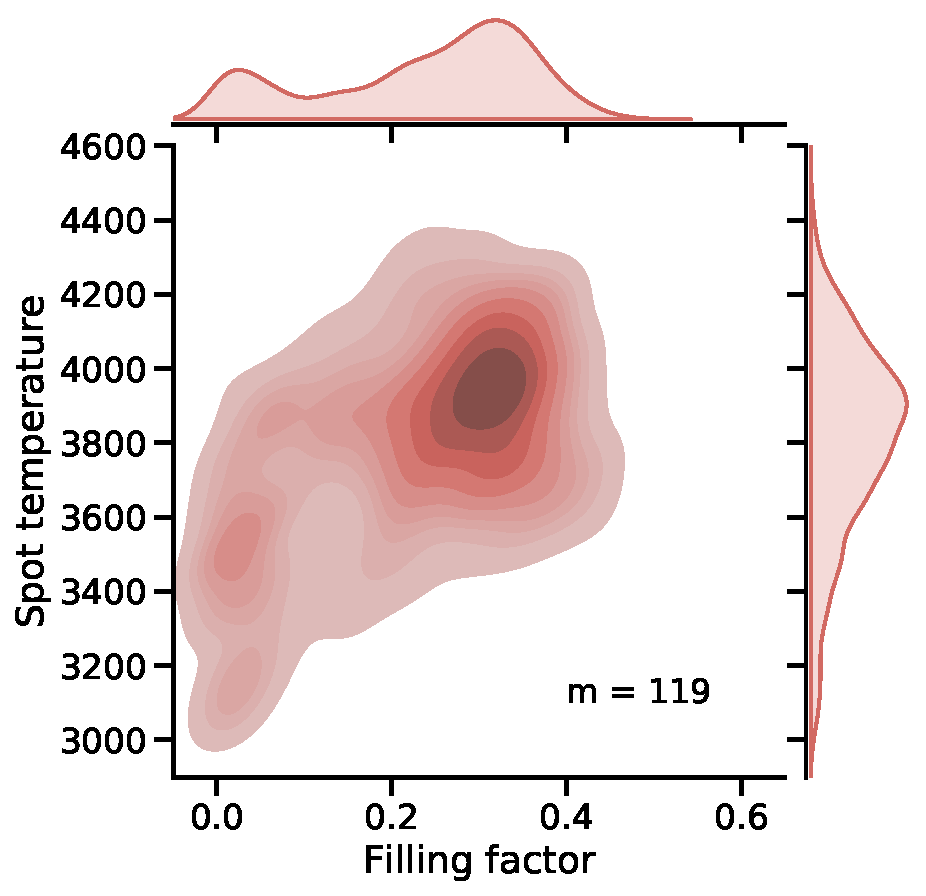
\includegraphics[width=2in]{figures/H_band_Tspot_fillingfactor_m119_new.pdf}} &
     \subfloat{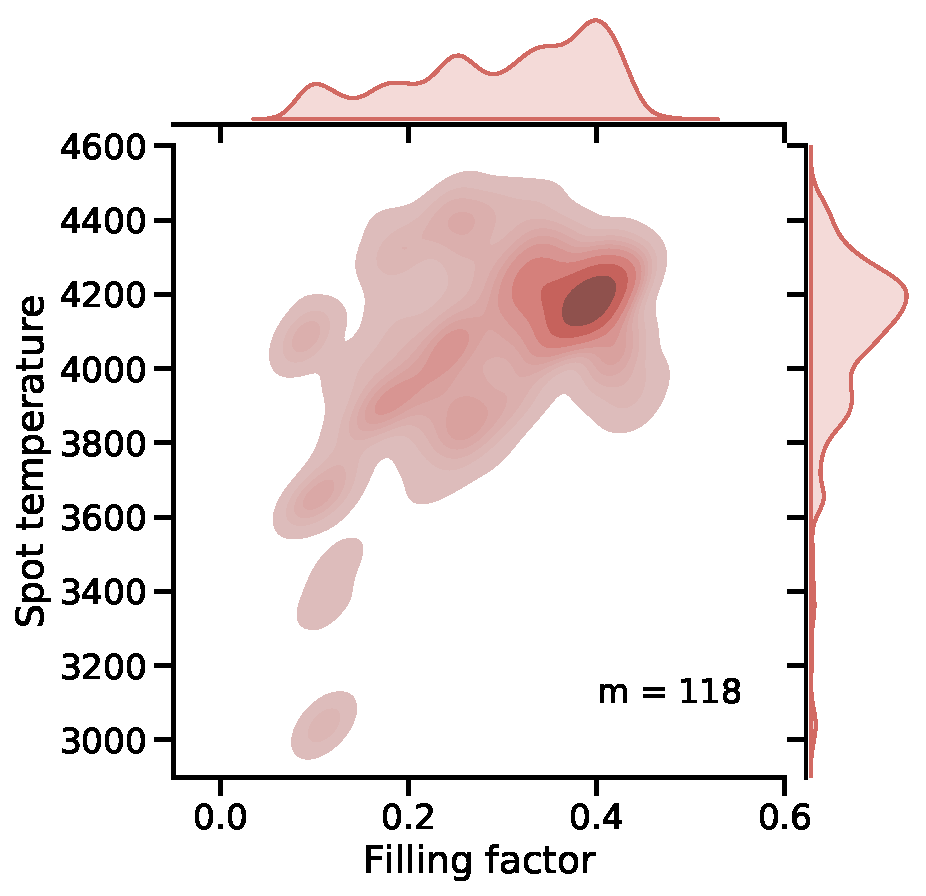
\includegraphics[width=2in]{figures/H_band_Tspot_fillingfactor_m118_new.pdf}} &
     \subfloat{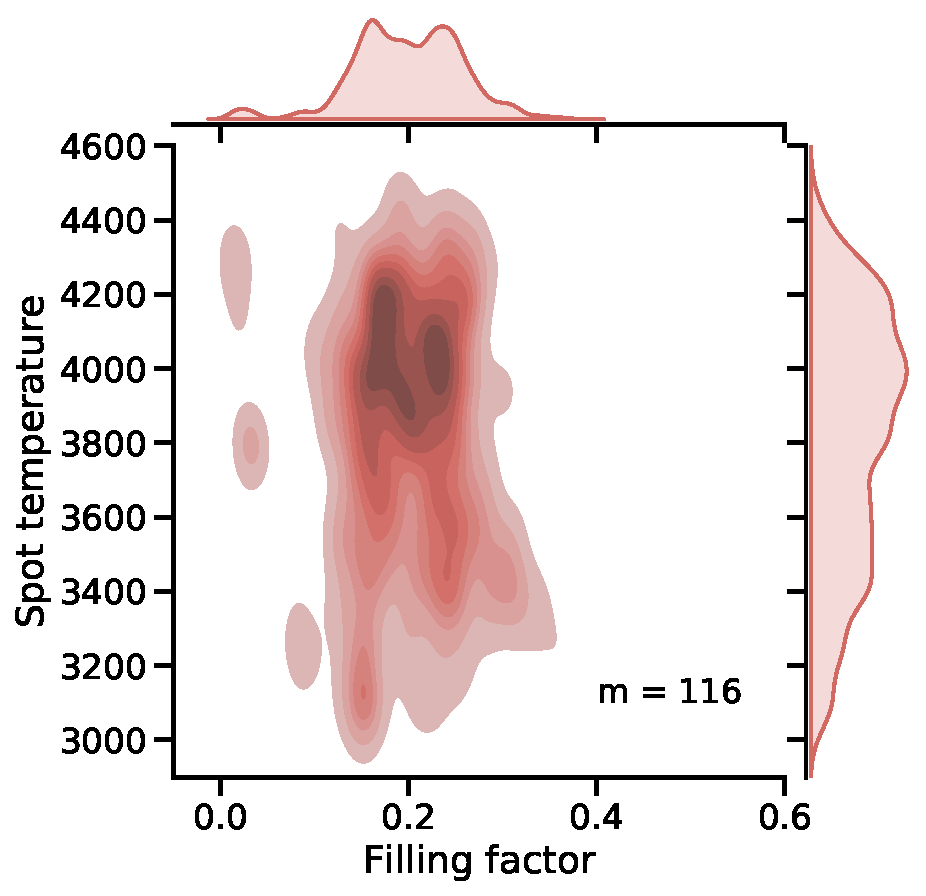
\includegraphics[width=2in]{figures/H_band_Tspot_fillingfactor_m116_new.pdf}} \\
     \subfloat{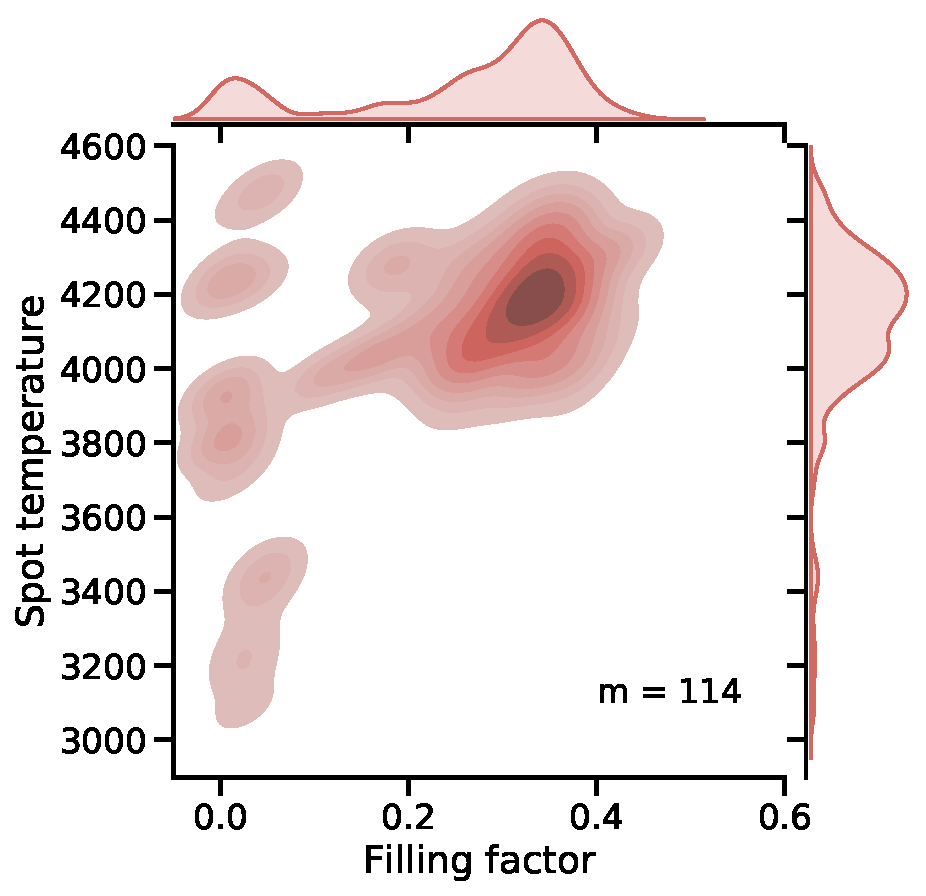
\includegraphics[width=2in]{figures/H_band_Tspot_fillingfactor_m114_new.pdf}} &
     \subfloat{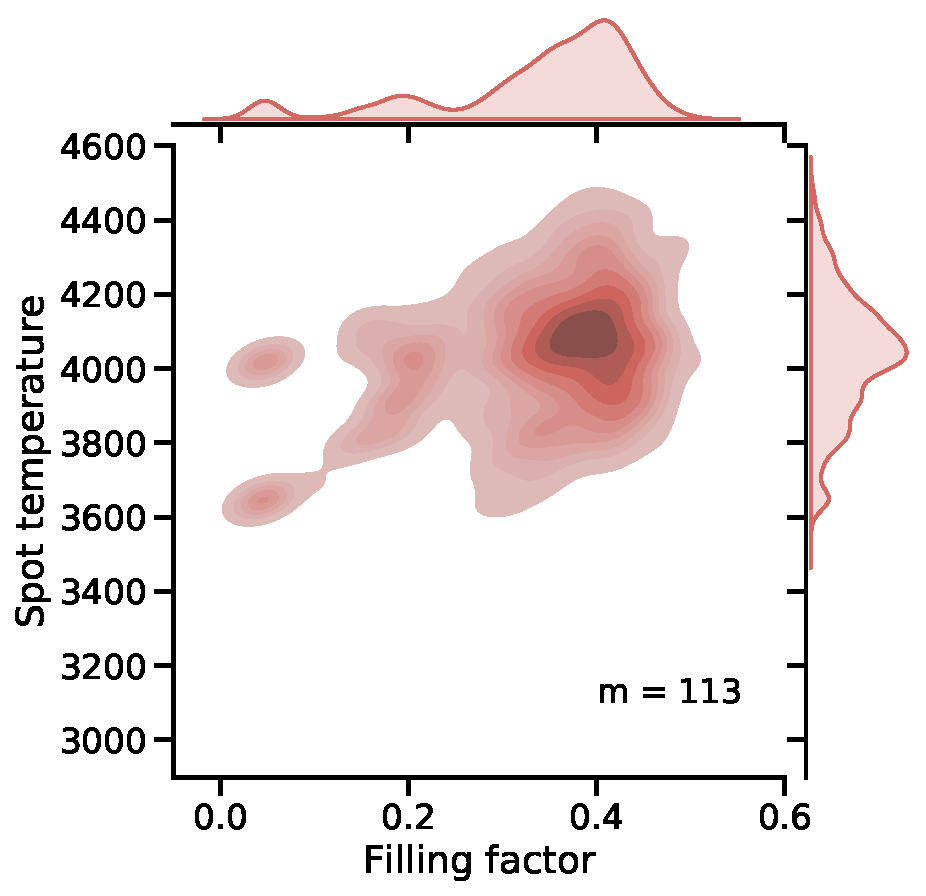
\includegraphics[width=2in]{figures/H_band_Tspot_fillingfactor_m113_new.pdf}} &
     \subfloat{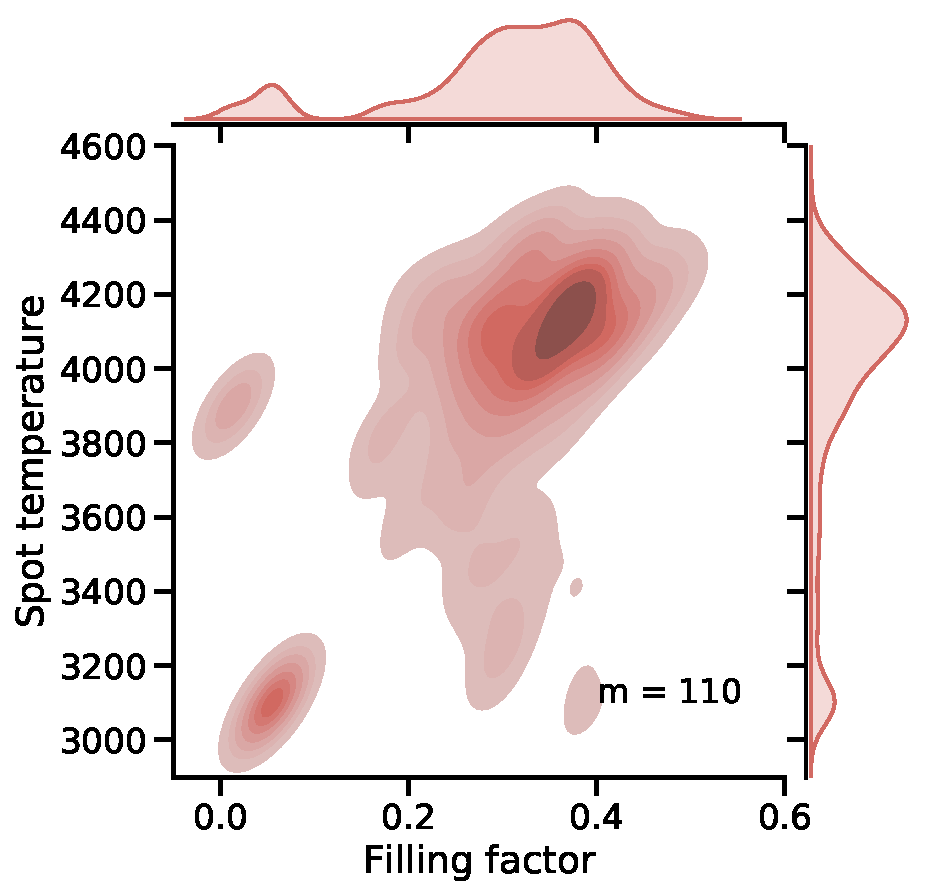
\includegraphics[width=2in]{figures/H_band_Tspot_fillingfactor_m110_new.pdf}} \\
     \subfloat{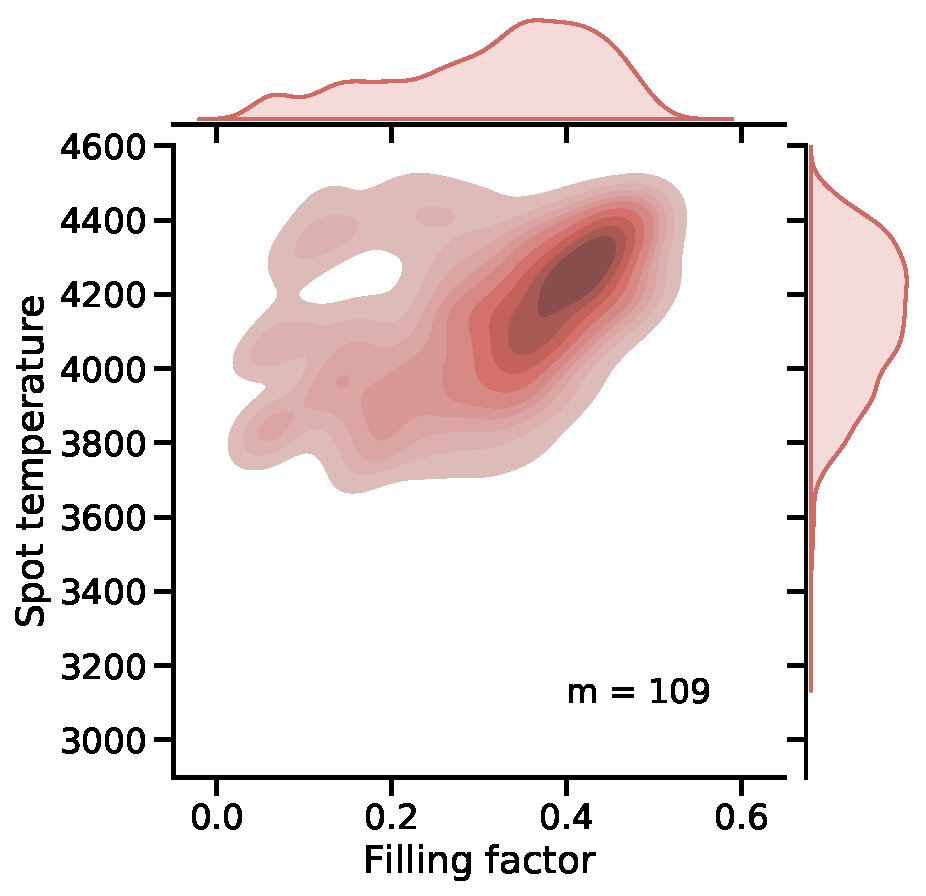
\includegraphics[width=2in]{figures/H_band_Tspot_fillingfactor_m109_new.pdf}} &
     \subfloat{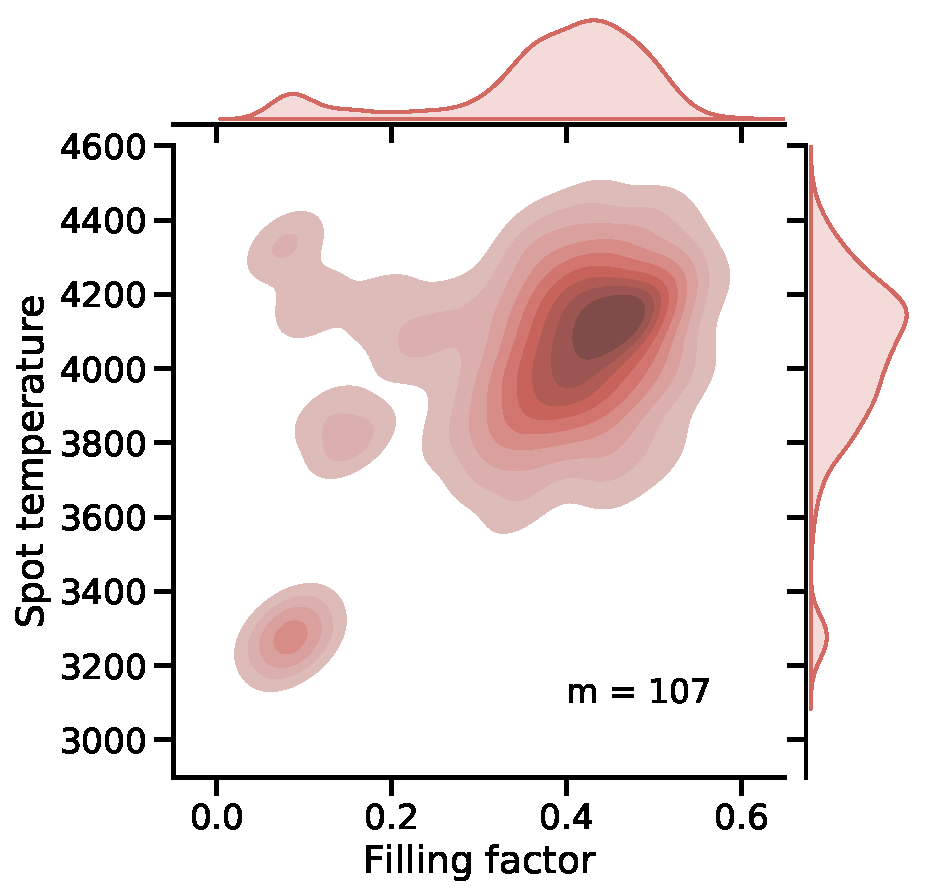
\includegraphics[width=2in]{figures/H_band_Tspot_fillingfactor_m107_new.pdf}} &
     \subfloat{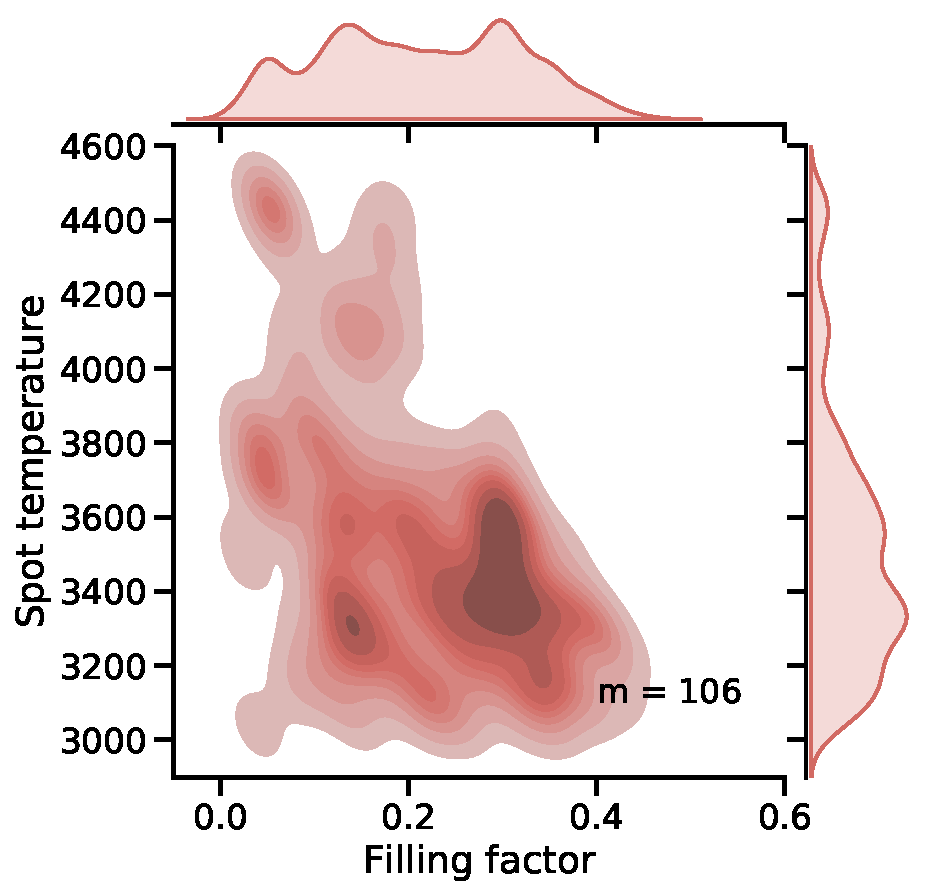
\includegraphics[width=2in]{figures/H_band_Tspot_fillingfactor_m106_new.pdf}}
   \end{tabular}
 \caption{2-dimensional distributions of filling factor and spot temperature for the nine accepted IGRINS orders for S1063, including 1000 samples of the emcee chains thinned by a factor of 10. Some orders demonstrate a stronger ability to constrain the spot characteristics than others, however all are consistent with the detection of a moderate covering fraction of spots. The median filling factor across these nine orders is $32 \pm 7$\% with a spot temperature of $4000\pm200$ K.}
 \label{fig:tspot_fillingfactor3x3}
 \end{figure*}
 
 \subsection{Comparison to evolutionary models of active stars}
 \label{sec:model_comparison}

\begin{figure*}[ht]
    \centering
    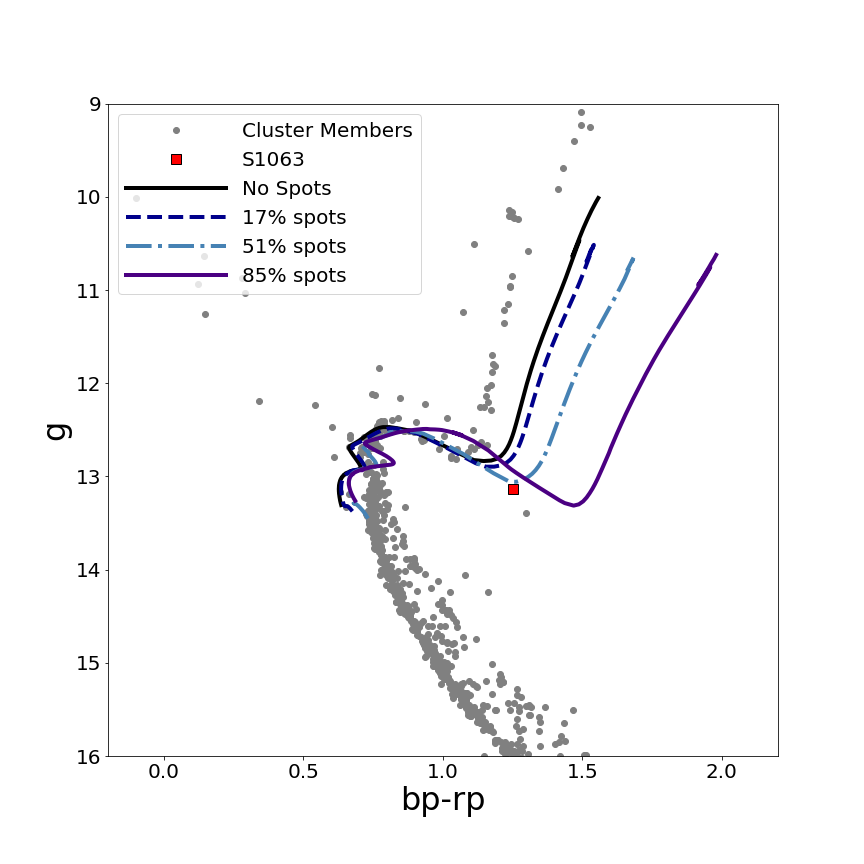
\includegraphics[width=0.45\linewidth]{figures/S1063_GaiaCMD.png}
    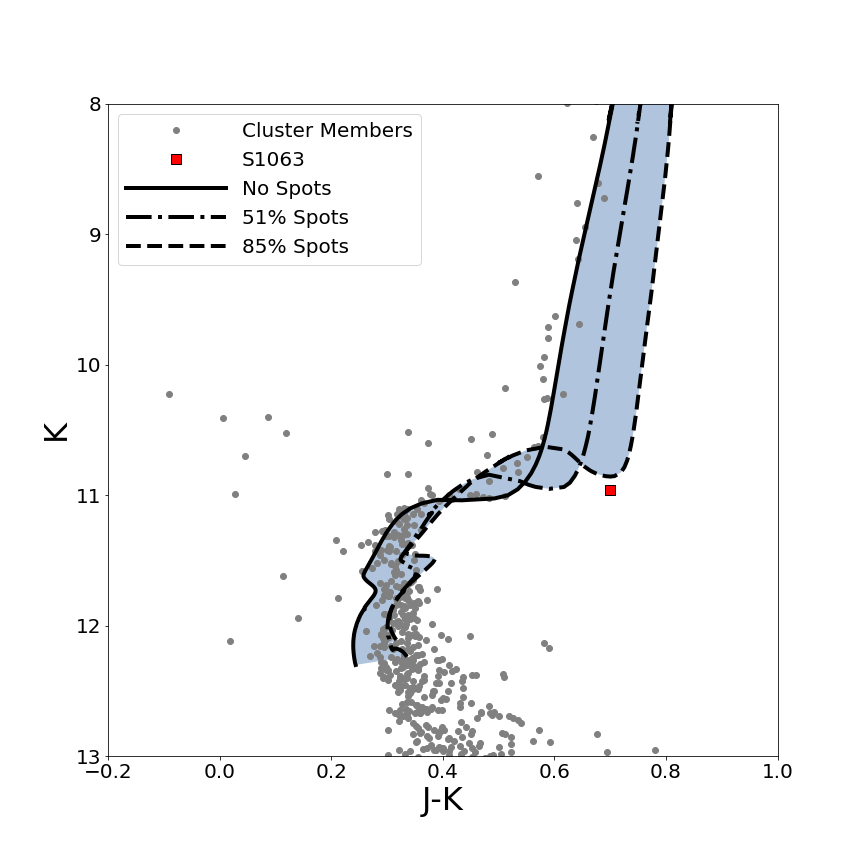
\includegraphics[width=0.45\linewidth]{figures/S1063_2MASS_CMD.png}
    \caption{On the left is a \textit{Gaia} color-magnitude diagram (CMD) that shows members of M67 (gray points) with SSG S1063 highlighted (red square). In comparison, we show SPOTS evolutionary tracks \citep{somers20} for a 1.3 \Msolar\ star with spot covering fractions of 0\%, 17\%, 51\% and 85\%. On the right is a similar CMD using photometry from 2MASS.}
    \label{fig:CMDs}
\end{figure*}

Current theoretical modeling of active stars take several different approaches, including surface treatments of spots at non-zero temperatures that suppress convective energy transport \citep{somers20}, direct treatments of the interior magnetic field \citep{2013ApJ...779..183F}, and reduced mixing length models with non-emitting spots \citep{2007A&A...472L..17C}. 

Here, we compare the photometry of S1063 to spotted SPOTS evolutionary tracks \citep{somers20}.  We use optical photometry from \textit{Gaia} and near-infrared photometry from 2MASS for this comparison, showing CMDs of M67 members compared to SPOTS tracks in Figure~\ref{fig:CMDs}. The optical photometry is most consistent with a SPOTS model with a $\sim50\%$ spot filling factor, slightly higher than the $32\%$ we find from the spectroscopic de-convolution. The 2MASS photometry indicates an even larger filling factor, falling in between the 51\% and 85\% SPOTS models. We note that while the unspotted SPOTS evolutionary track (black line in Figure~\ref{fig:CMDs}) fits the turnoff of M67 well when using 2MASS photometry, the model has a more extended subgiant branch and redder giant branch compared to the \textit{Gaia} photometry. This discrepancy is not resolvable by changing cluster parameters (i.e. reddening, distance, turnoff mass, metallicity). It may be due to internal model physics (i.e. choice of mixing length) or an error introduced when calculating model colors in the Gaia bandpasses. Because of this improper calibration, the spot filling factor inferred from comparisons with the \textit{Gaia} photometry may be skewed towards lower spot filling factors. This could explain the higher spot filling factor inferred from the 2MASS photometry, where the unspotted models are a better fit to the cluster turnoff. 

A summary of the surface and stellar parameters for S1063 are given in Table~\ref{tab:s1063parameters}, comparing our work here with parameters for S1063 determined in \citet{mathieu03}, \citet{leiner17}, and the SPOTS model comparison above. The filling factor determined via spectroscopic and photometric methods varies dramatically, with photometric methods finding a larger filling factor than our work here, although different photometric colors combinations suggest different filling factors. 

The spectral decomposition technique used here is sensitive to larger spot filling factors \citep{gullysantiago17}, as long as the spots are of sufficient brightness to provide a significant spectral signature. We detect a significant spot spectral signature in S1063, but we do not know if we are detecting the spectrum of the umbra or prenumbra. Although it is most likely that the penumbra is larger in area and warmer than the umbra for most stars \citep{1981ApJ...250..327V}, suggesting that this technique is more sensitive to constraining the prenumbra filling factor and the prenumbra would dominate the total spot area on the star. However, if SSGs have smaller penumbra it is possible this technique would under-sample the total spot coverage on the stellar surface. Additionally, any possible wavelength dependence of spot size would also lead to discrepant spot filling factors across photometric and spectroscopic determinations at different wavelengths. We note that photometry collected at different epochs can also impact the inferred photometric filling factor, but given our light curve analysis we expect epoch-based filling factor uncertainties to be at most $\sim$20\% in filling factor. 

We present further discuss systematic uncertainties that may add to these discrepancies in Section~\ref{sec:uncertainties}, but fully resolving the complexities of photometric and spectroscopic constraining of spot filling factors likely requires careful photometric modeling of a multi-temperature stellar surface, which is beyond the scope of this paper. 


\section{Discussion}
\label{sec:discussion}

The spot coverage fraction determined in this work is consistent with the range of spot coverage seen on RS CVn of 30--40\% from measuring TiO band strength \citep{oneal96, oneal98, oneal04} and Doppler imaging \citep{hackman12}. The similar spot coverage fraction on S1063 determined here is further evidence that this sub-subgiant and likely other sub-subgiants have high magnetic activity.

Strong magnetic fields and starspots reduce convective energy transport efficiency, which in turn mutates theoretical evolutionary model tracks from their unspotted/non-magnetic counterparts \citep{2013ApJ...779..183F,somers15,somers15b,somers20}. Understanding the physical nature of the magnetic activity and the impact it has on stellar structure and evolution requires comparison of high fidelity observations with these theoretical models.  An accurate position in the HR diagram position requires determination of the effective temperature ($T_{\textrm{eff}}$) having accounted for spots, as well as the stellar luminosity.

\subsection{Effective temperature of spotted stars}
The conventional observational interpretation of $T_{\textrm{eff}}$ is difficult to apply to spotted stars, especially stars with variation in the spot covering fraction over time \citep{gullysantiago17}.  Conventionally, a spectrum can be interpreted as possessing a 1:1 mapping from its appearance to a $T_{\textrm{eff}}$-indexed template, which can be either model-based or observed.  We...

\citet{leiner17} fit the multi-band spectral energy distribution for S1063 with a single Castelli-Kurucz spectrum \citep{2003IAUS..210P.A20C} and find a best fit $T_{\textrm{eff}}$ of 4500 K. Knowing we are dealing with a spotted star, another interpretation is to calculate the surface-averaged $T_{\textrm{eff}}$:

\begin{equation}
T_{\textrm{eff}}^4 = f_{\textrm{s}} T_{\textrm{s}}^4 + (1 -f_{\textrm{s}}) T_{\textrm{amb}}^4 .
\end{equation}

where $f_{\textrm{s}}$ is the spot covering fraction, $T_{\textrm{s}}$ is the spot temperature, $T_{\textrm{amb}}$ is the ambient photosphere temperature. This single surface-averaged temperature allows for comparisons to one-dimensional stellar evolution models motivated by the surface conditions of the star \citep{somers20}. With this method, at the time of the IGRINS observation the $T_{\textrm{eff}}$ of S1063 is $4900\pm100$ K. This temperature is inconsistent with the temperature determined via SED fitting in \citet{leiner17}, indicative of the discrepancies between the spectral and photometric constraints outlined in Section~\ref{sec:model_comparison}, although we note that the previous temperature of 4500 K is between the measured spot and ambient photosphere temperatures determined in this work.

Stars such as S1063, however, have observed surface-averaged $T_{\textrm{eff}}$ values that vary based on the spot covering fraction at the time of observation. We know from the variable light curve that stars such as S1063 have differing spot covering fractions on opposite observable hemispheres of the star causing optical variability. For example, at the 4-year light curve maximum when S1063 had approximately a 20\% spot covering fraction the surface-averaged $T_{\textrm{eff}}$ for the observed hemisphere of the star would be 5000 K. At the light curve minimum with a 45\% spot covering fraction the surface-averaged $T_{\textrm{eff}}$ for the observed hemisphere would only be 4700 K. 

The true surface-averaged $T_{\textrm{eff}}$ includes the entire stellar surface. This should be constant over a thermal timescale, including the four-year time frame in Figure~\ref{fig:lightcurve}, as is demonstrated by the constant mean flux level of 89.5\% compared to the maximum global flux. Observationally constraining the surface-averaged $T_{\textrm{eff}}$ requires either multi-epoch spectrum observations at both the light curve maximum and minimum, or a single observation at the mean flux level. The date of the IGRINS observation corresponds to a global flux level of 0.912, suggesting that observed spot coverage is a reasonable proxy for the mean state of S1063. Therefore, we conclude that the total surface-averaged $T_{\textrm{eff}}$ of S1063 is consistent with the observed surface-averaged $T_{\textrm{eff}}$ of $4900\pm100$ K. We stress, however, that determining a single $T_{\textrm{eff}}$ value for spotted stars is fraught at best, and makes model comparisons exceedingly nuanced.  


\subsection{Radius of S1063}

The radius of S1063 gets encoded into our data streams in three ways.  Kinematically, radius affects $v\sin{i}$, photometrically radius affects the SED and HR diagrams, and gravitationally radius affects the surface gravity $\log{g}$.  Our weak constraints on surface gravity cannot meaningfully inform the radius.  The SED-based photometric results suggest a radius of $R_{\star} = 3.7-4.6 R_\odot$, implausibly large compared to even the most egregiously spotted radii inflation models.  The kinematic avenue therefore seems most promising and ostensibly least subject to astrophysical biases, so it is worth dissecting in some detail here.  The stellar radius $R_{\star}$ contributes to the magnitude of the equatorial velocity $v_{\mathrm{eq}}$ for a given rotation rate and projected stellar inclination angle $i$:
\begin{eqnarray}
  v \sin{i} = \frac{2\pi R_{\star}}{P_{\mathrm{rot}}} \sin{i} \\
  R_{\star} \sin{i} = \frac{v \sin{i} \cdot P_{\mathrm{rot}}}{2 \pi} \\
\end{eqnarray}

Our \texttt{Starfish}/IGRINS-derived $v\sin{i}=XX$ and \texttt{celerite}/K2 derived period $P_{\mathrm{rot}}=XX$ constrain $R\sin{i} = XX$, with a formal statistical uncertainty of XX.  At first sight, $R_{\star}$ is most likely $>XX R_{\odot}$, since $\sin{i}$ is only ever less than unity.  The combined $XX\%$ uncertainty in $R\sin{i}$ and the photometrically-derived radius uncertainty of $XX\%$ yields coarse agreement/disagreement with these two disparately-sourced estimates. At least three sources of unaccounted-for astrophysical uncertainties can conceivably bias the derived $v\sin{i}$ for heavily spotted sub-giants.  The unknown limb-darkening prescription, the micro- or macro- turbulent velocity, and the latitudinal segregation of starspots.  On the other hand, the period can be systematically biased in three significant ways: differential rotation combined with latitudinal starspot segregation, starspot evolution on timescales comparable to the rotation period, and aliasing from regularly-spaced longitudinal surface symmetries.

\natalienote{
-Rsini can also be used as a model comparison, but this Rsini is large (we think 3.7-4.6 Rsun) compared to what has been found in previous SED fits (Leiner2017)}

%{f the with direct predictions for spot covering fractions of photometrically emitting spots. A preliminary comparison to S1063 is included in \citet{somers20}, but using a lower $T_{\textrm{eff}}$ as found in \citet{leiner17}. However, \citet{somers20} uses the surface-averaged temperature to define $T_{\textrm{eff}}$ (see Eq 1 in Somers20), so the $T_{\textrm{eff}}$ determined in this work is a more appropriate comparison.

%-Updated temp brings these results more in line with the spot coverage implied by SPOTS models, assuming the luminosity is the same. SPOTS models are maybe still a little bit too spotted - close to the 51\% track compared to 32\% that we measure, but our uncertainties are large and we have systematic errors that are unaccounted for.

%-Now there is tension with the colors of the SPOTS models, but colors of spots are weird. The lower spot coverage models predict bluer colors than observed. Perhaps some chromospheric component? This is probably fine.

%-Perhaps demonstrates a need for a dual modeling approach of surface treatment with internal structure changes and comparing against a larger sample of stars




\subsection{Additional sources of systematic uncertainty}
\label{sec:uncertainties}
We have posited a two-temperature surface two derive our estimates for filling factors and effective temperature.  In reality, this star---and most active stars more generally---must exhibit a range of apparent surface contrasts attributable to umbra, penumbra, faculae, chromospheric emission, and other phenomena unaccounted for in this work \citep{berdyugina05, 2009A&ARv..17..251S}.  

Our near-IR spectral technique is most sensitive to detecting a ``sweet-spot'' in starspot contrast: cool enough to exhibit a spectrum that is qualitatively distinct from the ambient photosphere, but not so cool as to possess vanishing specific intensity.  So for example, our technique might readily perceive the penumbra of the starspot, while ignoring the much cooler and darker umbra flux contribution \citep{1981ApJ...250..327V}.  This umbral neglect would lead our technique to systematically underestimate the total starspot coverage, rendering our claimed estimate as a lower limit.  On the other hand, faculae and plage act to add a hotter-than-average surface component.  The interpretation of our two component mixture model becomes confounded if we posit the coexistence of three components: spot, ambient, and faculae \citep{1998A&A...329..747S}.  The extent of the confounding depends on the detailed properties of such conceivable faculae, but in short faculae may act to either increase or decrease starspot coverage estimates insofar as they alter the ambient photosphere temperature that we assign \citep{2019AJ....157...11W}.  The existence of large and hot faculae can be ruled out to some extent by the fact that they would dominate the temperature determination in visible wavelength spectra.  The adequate agreement temperature derived from visible wavelength spectra of S1063 \citep{mathieu03} and the our near-IR derived ambient photosphere temperature suggests that faculae may be negligible.  Chromospheric emission should mostly perturb individual lines that are known to be chromospherically active, such as Hydrogen lines.  Our IGRINS-based technique analyzed the majority of the $H$-band with whole-spectrum fitting, where such chromospherically active lines would have negligible impact.

Our reliance on \texttt{PHOENIX} synthetic spectra adds a model-dependent systematic to our entire approach.  The unavailability of a large number of spot-free high-precision high-resolution template spectra across all of $H$-band demands the use of these models in order to compare to IGRINS data.  The ability of such synthetic spectra to resemble starspots remains an unknown.  We can get some clue of the performance of the synthetic spectra by examining the fit residuals, evinced in this work by comparing the purple two-component composite spectrum to the gray IGRINS spectrum in Figure \ref{fig:IGRINS_spectra3x3}. The IGRINS spectra exhibit absorption lines where no such line is predicted, and vice versa: lines absent from the IGRINS spectra that our composite model would predict.  To some extent, the imperfect fitting of the synthetic spectra to our IGRINS spectra must be causing a systematic uncertainty.  The Gaussian process ``Global Kernels'' employed in \texttt{Starfish} account for some degree of correlated data-model residual mismatching.  We did not employ the ``Local kernels'', which cause a 30 K systematic bias in comparable quality spectra of WASP-14 also compared to the \texttt{PHOENIX} models \citet{czekala15}.  We therefore assign at least a 30 K systematic bias in our temperature estimates based on the prospect of individual line outliers polluting our fit residuals.  We conseassign a coarse estimate of 100--200 K to so-called ``label noise'', associated with the alignment of a best fit \texttt{PHOENIX}-provided $T_{\text{eff}}$ labels and an unseen ground-truth label for the ``True'' temperature of the spots. New studies of the Sun based on DKIST may offer the best future avenue for testing such assumptions and refining the ability to distinguish starspot emission from ambient photosphere.


%%% TODO: retool below discussion for the HRD discussion
%\subsection{Starspots as confounding factors}
%Mass, age, and metallicity uniquely map a main sequence star to its HR diagram position.  A fourth factor---rotation---confounds this mapping in as-yet-unknown ways.  Rotation might enhance spread in HR diagram positions (cite XX Davenport, Douglas?), with the most conspicuous spreads in the pre-main sequence regime (cite XX Covey, Stauffer).  Spreads in the HR diagram offer clues to the consequences of rotation.  Increased rotation heightens the magnetic dynamo strength and concomitant surface magnetic field.  These magnetic fields suppress convective efficiency, meaning the star must increase in size at a lower effective temperature to allow the same amount of internal energy to escape (cite XX Feiden): rotating stars become bigger and cooler than their non-rotating counterparts (cite XX Somers).  The interplay of rotation, dynamo, and surface fields remain an active area of research, with bright prospects for a unified theory involving the degree of magnetic complexity parameter (cite XX Garraffo).

%Surface magnetic fields offer two key observational manifestations.  The Zeeman Effect splits spectral line levels in magnetic-sensitive atomic transitions (cite XX Johns-Krull).  Starspots induce stellar surface inhomogeneities that can be seen in the modulation of

%The story in the post-main sequence is less clear.  Angular momentum transport governs rotation  as stars evolve over orders of magnitude in size.




%In the absence of this spectral inference technique one could assume the \textit{K2} C5 light curve maximum corresponded to zero spot presence with the light curve amplitude change implying a maximum spot coverage of 7--10\%. This provides a fundamentally different view of the star ...

%\begin{itemize}
%\item Conceivable geometries with circumpolar active longitudes, or migrating active latitudes
%\item Biases introduced if we assume a spot-free model
%\begin{itemize}
%  \item Where does subsub sit in a new HR diagram? (new Somers models)
%  \item *bonus* FIGURE: PMS HR diagram with new Somers tracks
%  \item Spot impact on SED fits
%\end{itemize}
%\end{itemize}

\section{Conclusions}
\label{sec:conclusions}

Reiteration here.

\clearpage
\pagebreak


%\appendix
%\section{Appendix heading}
%\label{methods-details}
%Placeholder text

\begin{acknowledgements}

%ADS
This research has made use of the NASA Astrophysics Data System.
%IGRINS
This work used the Immersion Grating Infrared Spectrometer (IGRINS) that was developed under a collaboration between the University of Texas at Austin and the Korea Astronomy and Space Science Institute (KASI) with the financial support of the US National Science Foundation under grant AST-1229522, of the University of Texas at Austin, and of the Korean GMT Project of KASI.
%Kepler
This paper includes data collected by the Kepler mission. Funding for the Kepler mission is provided by the NASA Science Mission directorate.
% MAST
Some of the data presented in this paper were obtained from the Mikulski Archive for Space Telescopes (MAST). STScI is operated by the Association of Universities for Research in Astronomy, Inc., under NASA contract NAS5-26555.

%gaia
This work has made use of data from the European Space Agency (ESA) mission
{\it Gaia} (\url{https://www.cosmos.esa.int/gaia}), processed by the {\it Gaia}
Data Processing and Analysis Consortium (DPAC,
\url{https://www.cosmos.esa.int/web/gaia/dpac/consortium}). Funding for the DPAC
has been provided by national institutions, in particular the institutions
participating in the {\it Gaia} Multilateral Agreement.

\end{acknowledgements}

\facilities{Smith (IGRINS), Gaia, ASAS}

\software{  pandas \citep{mckinney10},
  emcee \citep{foreman13},
  matplotlib \citep{hunter07},
  numpy \citep{2020NumPy-Array},
  scipy \citep{2020SciPy-NMeth},
  ipython \citep{perez07},
  starfish \citep{czekala15},
  seaborn \citep{waskom14},
  lightkurve \citep{geert_barentsen_2019_2565212}}

\clearpage

\bibliography{ms}

\end{document}
